% ---------------------------------------------------------------------------- %

\section{Prototipagem da Interface de Utilizador}
\label{cap:interface}

Antes de se proceder à modelação da arquitetura interna do sistema, construiu-se um protótipo da interface de utilizador disponibilizada pelo sistema, o qual é descrito neste capítulo.

% ---------------------------------------------------------------------------- %

Quando a aplicação é iniciada, são requisitas as credenciais, nome de utilizador e palavra-chave, para a autenticação do utilizador. É fornecida também a opção de criar uma conta pessoa. A criação de uma conta requer, para além das informações necessárias à autenticação, a confirmação da palavra-chave e opcionalmente a introdução de um endereço de \emph{email}. Estas duas funcionalidades podem ser observadas na \reffig{fig:interface:login} e \reffig{fig:interface:registar}.

\begin{figure}[H]
  \centering 
  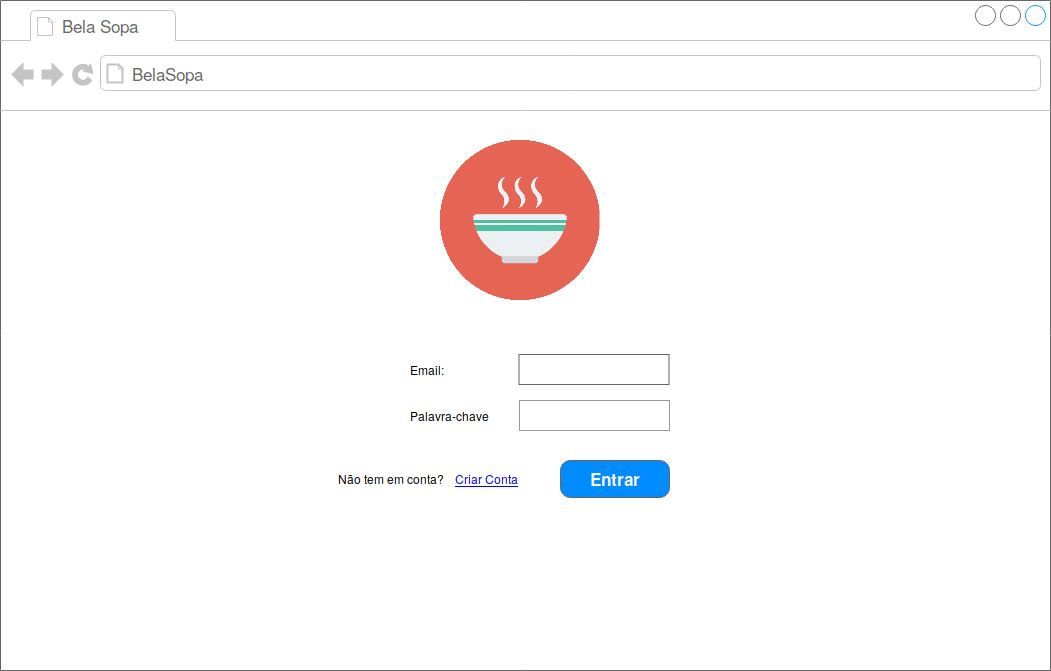
\includegraphics[width = \textwidth]{figures/07/Login.png}
  \caption{Protótipo da interface de autenticação.}
  \label{fig:interface:login}
\end{figure}

\begin{figure}[H]
  \centering 
  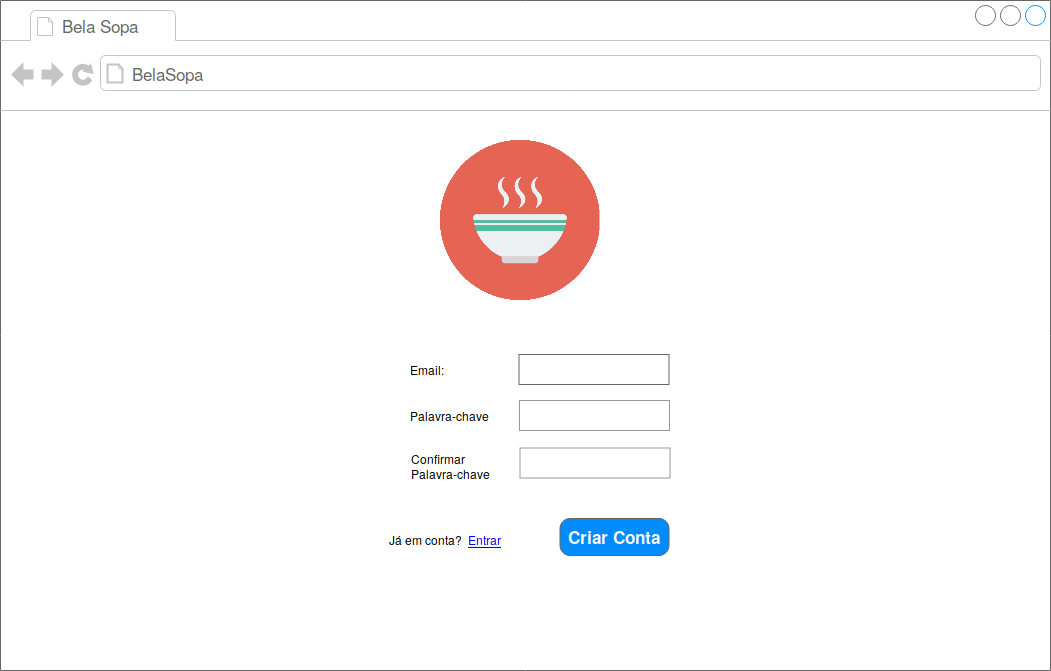
\includegraphics[width = \textwidth]{figures/07/Registar.png}
  \caption{Protótipo da interface de criação de contas.}
  \label{fig:interface:registar}
\end{figure}

Após a autenticação, é apresentado ao utilizador uma lista com todas as receitas do sistema. Nessa mesma janela é visível um menu lateral onde o utilizador pode aceder:
\begin{itemize}
    \item à sua conta pessoal;
    \item à receita que está em confeção (pode não estar visível);
    \item à lista de todas as receitas no sistema;
    \item à lista de todos os ingredientes no sistema;
    \item à lista de todas as técnicas no sistema;
    \item à lista de todos os ingredientes no sistema;
    \item à agenda semanal do utilizador;
    \item ao histórico do utilizador.
    \item à localização de lojas, \emph{Gota Doce}, próximas.
\end{itemize}
, tal como se apresenta na \reffig{fig:interface:paginicial}.

\begin{figure}[H]
  \centering 
  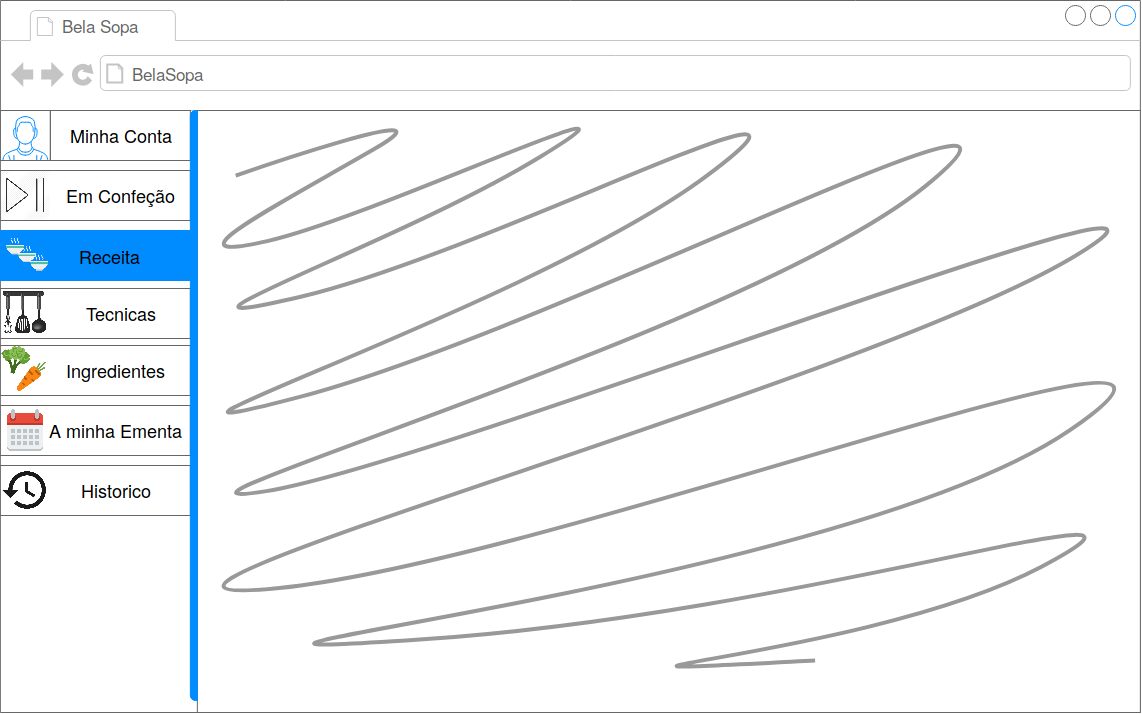
\includegraphics[width = \textwidth]{figures/07/PaginaInicial.png}
  \caption{Protótipo geral das interfaces de cliente.}
  \label{fig:interface:paginicial}
\end{figure}

A janela de pesquisa, dá a liberdade ao utilizador de pesquisar uma receita por nome, etiqueta ou por dificuldade. Depois do filtro ser ativado, são apresentadas todas as receitas que são validas de acordo com o filtro. Na apresentação das receitas, é apresentado uma imagem, titulo e etiqueta de cada receita, tal como se demonstra na \reffig{fig:interface:pesquisa}

\begin{figure}[H]
  \centering 
  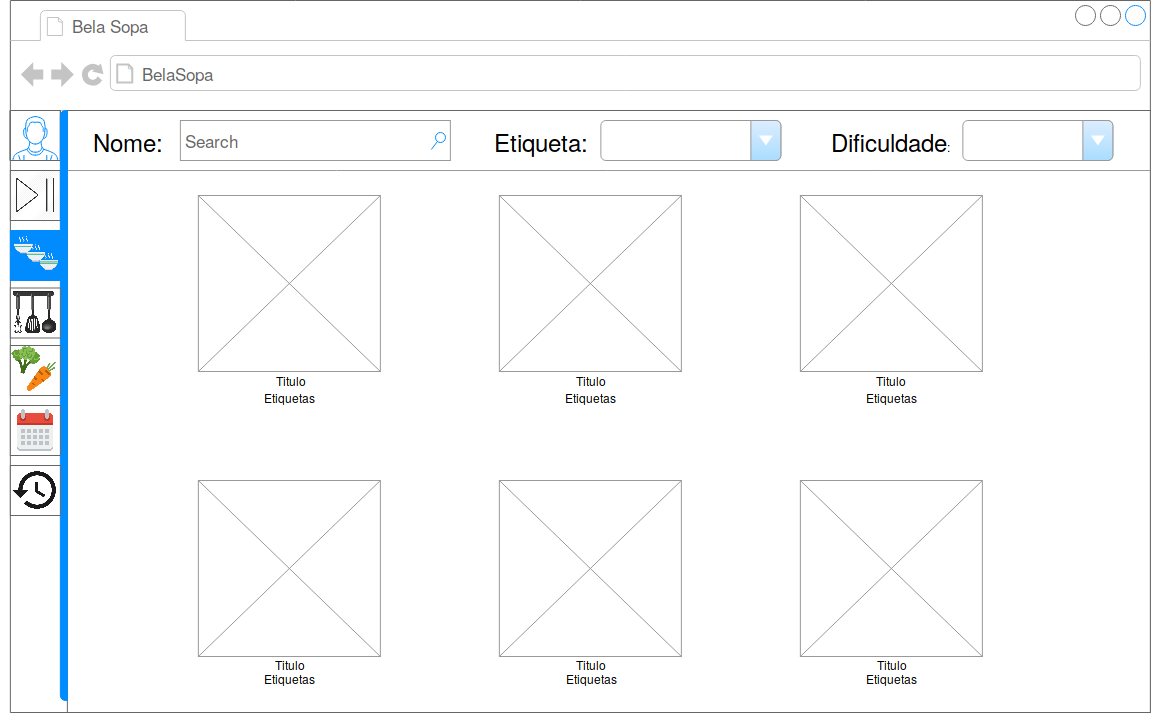
\includegraphics[width = \textwidth]{figures/07/Pesquisa.png}
  \caption{Protótipo da interface de listagem de receitas.}
  \label{fig:interface:pesquisa}
\end{figure}

Quando o utilizador seleciona uma receita, esta é apresentada como na \reffig{fig:interface:visualizacao}, ou seja, é apresentado uma imagem da receita, o titulo, uma breve descrição, a dificuldade, a etiqueta, a duração, a porção, a lista de todos os ingredientes e as suas respetivas quantidades, a lista de utensílios, a lista de técnicas, alista de tarefas e um conjunto de valores nutricionais.

\begin{figure}[H]
  \centering 
  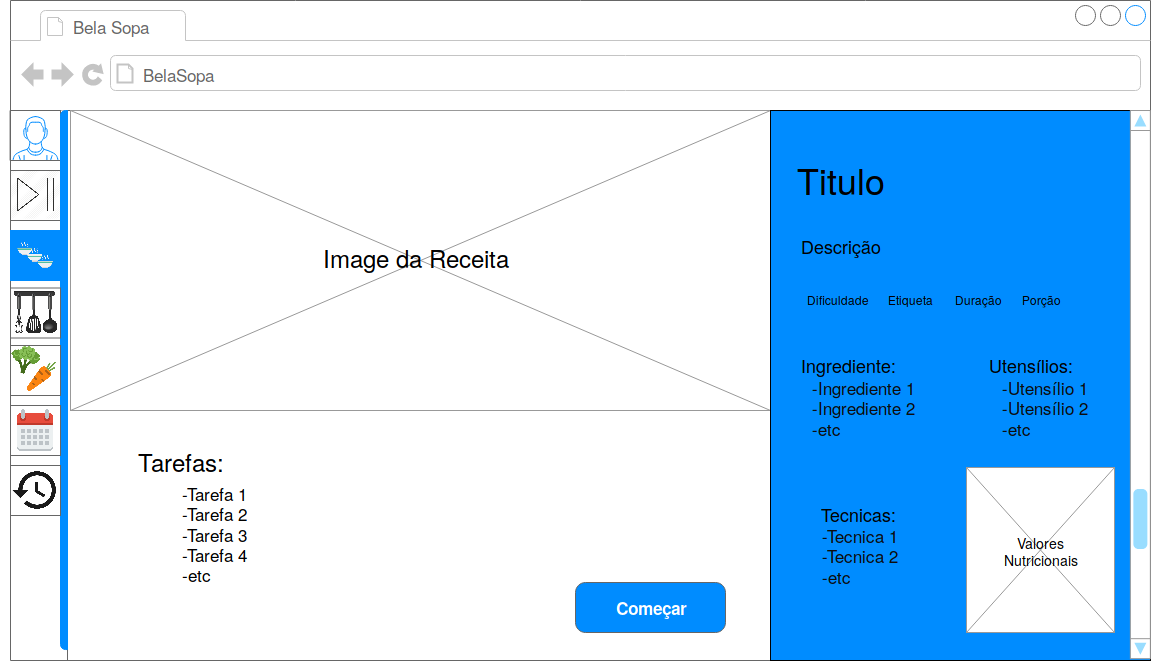
\includegraphics[width = \textwidth]{figures/07/Visualização.png}
  \caption{Protótipo da interface de visualização de uma receita.}
  \label{fig:interface:visualizacao}
\end{figure}
 
 Após iniciar a confeção, as informações da receita continuam a ser apresentados, exceto a lista de todos os ingredientes, de todos os utensílios e de todas as tarefas. Estas são reduzidas para cada processo, ou seja, em cada processo só são apresentadas as listas dos ingredientes, utensílios e tarefas referentes ao processo atual. Para alem dessas informações, a janela permite ao utilizador avançar para o processo seguinte, recuar para o processo anterior, cancelar a confeção e iniciar um temporizador, tal como demonstrado na \reffig{fig:interface:confecao}.

\begin{figure}[H]
  \centering 
  \includegraphics[width = \textwidth]{figures/07/Confeçao.png}
  \caption{Protótipo da interface de confeção de uma receita.}
  \label{fig:interface:confecao}
\end{figure}

%- Janela inicial
%    - Permite fazer login
%    - Permite registar conta de cliente

%- Janela depois de login de cliente
%    - Link para definições de conta
%    - Possibilidade de definir etiquetas pelas quais o cliente tem interesse
%    - Tab de histórico de receitas já confecionadas
%        - Incluindo dados ou estatísticas relativos aos cozinhados realizados
%    - Tab de receitas marcadas como favorito
%    - Tab de receitas
%        - Motor de busca de receitas por nome, por etiqueta
%        - Listagem de receitas por etiqueta
%    - Tab de técnicas
%        - Motor de busca de técnicas por nome
%    - Tab de configuração da ementa semanal
%        - Possibilidade de gerar lista de compras geral para uma dada semana

%- Janela de definições de conta de cliente

%    - Possibilidade de mudar passe e dados pessoais

%- Janela de receita

%    - Adicionar/remover aos/dos favoritos
%    - Adicionar à ementa semanal (especificar dia e tal)

%    - Descrição, imagens, etc.
    
%    - Porção (nº de comedores para as quantidades referidas nos passos e nos ingredientes necessários)

%    - Utensílios necessários (?)
%    - Ingredientes necessários e medidas
%    - Passos da receita
%        - Clicar no link de uma técnica no texto do passo para ver informação sobre a técnica
%    - Tempo de confeção
%    - Dificuldade
%    - Informação nutricional

%    - Link para ver Pingo Doces próximos e mostrar bing maps com percurso e tudo
%    - Link para redirecionar para loja para comprar ingredientes

%    - Começar confeção

%- Janela de confeção de receita

%    - Mesmas coisas que "janela de receita" e mais coisas
    
%    - Possibilidade de o utilizador especificar o passo em que se encontra / passos já realizados, etc.
    
%    - Os passos estão agrupados em grupos, cada grupo pode ter 1 ou mais passos, a ideia é que os passos dentro de um grupo possam ser efetuados "em paralelo", o passo atual é na verdade um grupo atual, os grupos inativos estão mais pequenos/mais cinzentos (para focar a atenção do utilizador)

% ---------------------------------------------------------------------------- %
